% !TEX TS-program = xelatex
% !TEX encoding = UTF-8 Unicode

\providecommand{\home}{../..}
\documentclass[\home/main.tex]{subfiles}

\begin{document}

\setlaymanexpl{We summarize our main findings from using simulation for robotic learning, developing smart textile, collecting a dataset and learning perceptual progression metrics.}

\chapter{Conclusion}\label{ch:conclusion}
% We review the main findings on using learning-based methods to solve fundamental problems in learning how to fold clothing items with robots. First, in \cref{sec:conc_challenges}, we recapitulate the main challenges associated with manipulating highly deformable objects. Next, we present the main contributions and findings of our research in \cref{sec:conc_research}. Finally, we provide our future perspectives on the field of robotic manipulation of deformable objects in \cref{sec:conc_future_work}.

% \section{Challenges in learning robotic folding} \label{sec:conc_challenges}
Deformable objects change shape on interaction. These changes lead to an infinite amount of configurations that need to be considered when manipulating deformable objects like clothing items. This is problematic as rigid body manipulation methods are not easily transferrable to objects that deform.
A solution for dealing with real-world variability is using learning-based methods by interacting with the environment. However, deep learning, the dominant learning paradigm, requires tremendous amounts of data to work. Several issues need to be addressed to effectively employ machine learning methods. These issues range from dedicated hardware for handling cloth to accelerating learning with priors to avoid generating months of training data on real robots.

\section{Research conclusions} \label{sec:conc_research}
In this research, we filled in gaps towards learning robotic folding of clothing items.
We started our dissertation by providing a self-contained chapter introducing the fundamentals of robotic manipulation of folding cloth (\cref{ch:lit}). We have discussed methodologies, tools and approaches to building a cloth folding pipeline while identifying strengths, weaknesses and gaps. This exposition gave rise to the motivations behind this research: \textbf{solving the lack of data and quick learning methods for learning to fold cloth.}

As a first solution to accelerating learning, we developed a cloth simulation environment (\cref{ch:simulation}). A salient feature of our cloth simulator is that it leverages \gls{GPU} acceleration, similar to how deep neural networks profit from concurrent calculations on \gls{GPU}. \textbf{Our robotic-cloth simulator successfully uses deep \gls{RL} to learn to fold a cloth two times, sequentially}. However, transfer to the real world is non-trivial as the simulation uses the cloth's full state, which is inaccessible in the real world.

To make state estimation of cloth possible in the real world, we developed a smart cloth (\cref{ch:instrumentation}). Our smart cloth employs off-the-shelve components and can be fabricated DIY and low-cost. It sandwiches a piezoresistive rubber between two layers of conductive threads, forming a grid of tactile cells. By recording a dataset of labelled cloth states, we demonstrate that standard machine learning methods can classify the cloth state. The main feature of our smart cloth is that it can serve as a state observation or reward function in an RL framework. In our experiments, we employ the smart cloth as a sparse reward function indicating whether the cloth is folded or not. Our results demonstrate that \textbf{our low-cost smart textile can learn to fold a cloth on a low-cost dual robotic arm platform in-vivo}.

Data is a critical element for building intelligent systems. Yet, the field of folding clothing is less endowed with datasets compared to its rigid body counterpart. For this reason, \textbf{we constructed a data collection setup to crowdsource a dataset of people folding clothing articles} (\cref{ch:data_collection}). The benefit of taking a citizen science approach to collecting our data is the diversity it generates in example demonstrations. Our dataset consists of roughly \qty{300000} multi-perspective RGBD images and is available online for researchers and practitioners to use. We labelled the frames to include pose information and annotated folding quality and substeps. With this dataset, we aim to fill in a gap in learning deformable objects manipulation, bootstrapped by human examples.

Learning from interaction with the environment, formalized by RL, is a potential way to acquire robotic manipulation skills as it shares principles with how humans learn skills. A major element is the reward function that signals how well an agent is solving the task. In the case of folding cloth, constructing a reward signal is non-trivial: it is required to measure the state of the cloth, including folds and wrinkles, and translate it to a scalar value. Although this engineering is possible with instrumentation (\cref{ch:instrumentation}), it is difficult to express how well a cloth is being folded. The field of RL solves this problem by considering the inverse problem: instead of finding the optimal policy using a reward function, what is the reward function given some optimal policy. However, inverse RL follows a computationally expensive approach by optimizing policy and reward simultaneously. For this reason, we decouple policy and reward learning. We have proposed \textbf{a method for learning reward functions in the form of progression metrics without labelling any data} (\cref{ch:reward_functions}). Our labelling-free approach is achieved by utilizing self-supervised learning on time as contrastive signal. We validated our method on the dataset collected in \cref{ch:data_collection}. Using case-based experiments, we have found that our method learns task-relevant features and useful invariances, making it robust to noise, distractors and variations in the task and shirts. The experimental results have shown that the proposed method can monitor processes in domains where state representation is inherently challenging, such as folding clothing items.

Finally, we have compiled our vision for future directions of the field of robotic folding (\cref{ch:towards_robotic_folding}). We have stressed the importance of democratized hardware, sensing, data and the integration between morphology and control.

\section{Future research directions} \label{sec:conc_future_work}
While \cref{ch:towards_robotic_folding} provided our high-level perspectives on the field of robotic folding,
% on the field of robotic folding, based on our experiences and research done in this work. 
% , we compiled our vision for future directions of the field of robotic folding.
this section zooms in on specific improvements and future directions for the methods and contributions of our research. We categorize future work in the following categories:
(a) extending our cloth folding dataset;
(b) improving the scope of our instrumentation process; and
(c) learning reward functions from demonstrations.

\subsection{Extending cloth folding dataset}
\Cref{ch:data_collection} introduced our crowdsourced dataset of humans folding clothing items.
As future work, the dataset can become a general-purpose cloth manipulation dataset. This is possible by adding novel clothing types to the set, such as trousers and socks.
We noticed in our reward function experiments (\cref{sec:rewards_discuss}) that the embedding is unable to distinguish small perturbations in the folds. Hence, adding a detailed view on the cloth being manipulated is useful in better identifying wrinkles and small perturbations on the cloth. This can be done by placing cameras with larger focal length focussed on the cloth. Alternatively, instrumented cloth (\cref{ch:instrumentation}) can be added to the mix to provide an extra source of modality.

Our dataset can also evolve to a benchmark for cloth state classification and action recognition.
A classification task can be added as a category to our folding dataset. A classification task of state configuration or tactile sensing reconstruction can be defined by recording the same clothing articles in different configurations, optionally with instrumentation. The clothing articles can optionally be linked to a virtual twin, using the cloth simulation we developed (\cref{ch:simulation}).
Eventually, these inclusions can lead to the dataset becoming a general benchmark instead of the role it now plays, i.e.\ providing example demonstrations to bootstrap learning.

\subsection{Instrumentation}
The smart textile introduced in \cref{ch:instrumentation} was improved by \textcite{Proesmans2022} to a modular, wireless sensing technology able to classify the state of larger cloths. With the availability of linking multiple sensing patches, future work can consider classifying more complex states, similar to the substeps defined in our dataset (\cref{ch:data_collection}), for example, left sleeve folded. An interesting follow-up is fusing the tactile information of the smart cloth with camera images in order to generate a multimodal database of self-labelled images of arbitrary cloth configurations. This data is produced by manipulating the cloth while recording its state with cameras. The multimodal dataset can then be used to learn a multimodal latent space as in \autocite{Lee2019}. We elaborate on this idea in the following section.

\subsection{Learning reward functions from demonstrations} \label{subsec:conc_future_tcn}
A key component in the reward learning framework proposed in \cref{ch:reward_functions} is the manner in which the embedding is trained. Training is done in a self-supervised way by building a dataset of anchor-positive-negative triplets from different perspectives using time as a contrastive signal. The central philosophy behind this training design is to learn useful invariances. By forcing two frames from a different viewpoint to be closer in embedding space than two temporal distant frames from the same viewpoint, we achieve viewpoint invariance. Similarly, we hypothesize that some form of input modality invariance can be learned by introducing different modalities. In this scenario, a camera image and tactile sensing of a cloth from the same timestamp should be closer in embedding space compared to the same camera image and the tactile input of the robot's finger from different timestamps. We visualize this idea in \cref{fig:conc_multimodal_tcn}. %An extra benefit of this proposal is dealing with missing values:    
Another approach to including multiple modalities is similar to the approach in \autocite{Lee2019}: different backbone architectures per modality fused into an embedding trained on pseudotasks like predicting optical flow and contact.

\begin{figure}[htpb]{}
    \centering
    \begin{subfigure}[b]{0.90\textwidth}
        \centering
        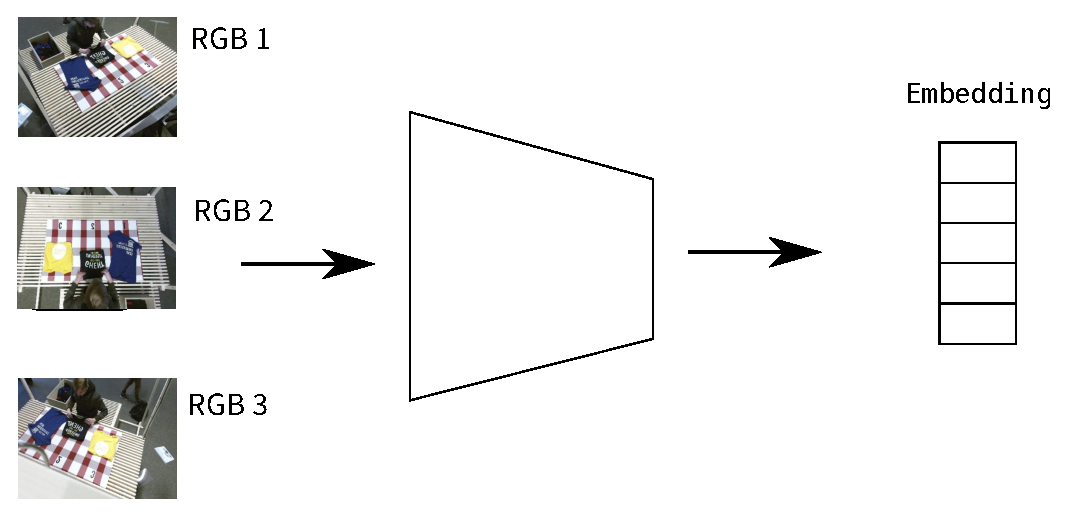
\includegraphics[width=\textwidth]{\home/chapters/08-conclusion/figures/ssr_nn_architecture_rgb}
        \caption{Three camera images from different perspectives as input.}
        \label{fig:conc_tcn_rgb}
    \end{subfigure}
    \par\bigskip % force a bit of vertical whitespace
    \par\bigskip % force a bit of vertical whitespace
    \begin{subfigure}[b]{0.90\textwidth}
        \centering
        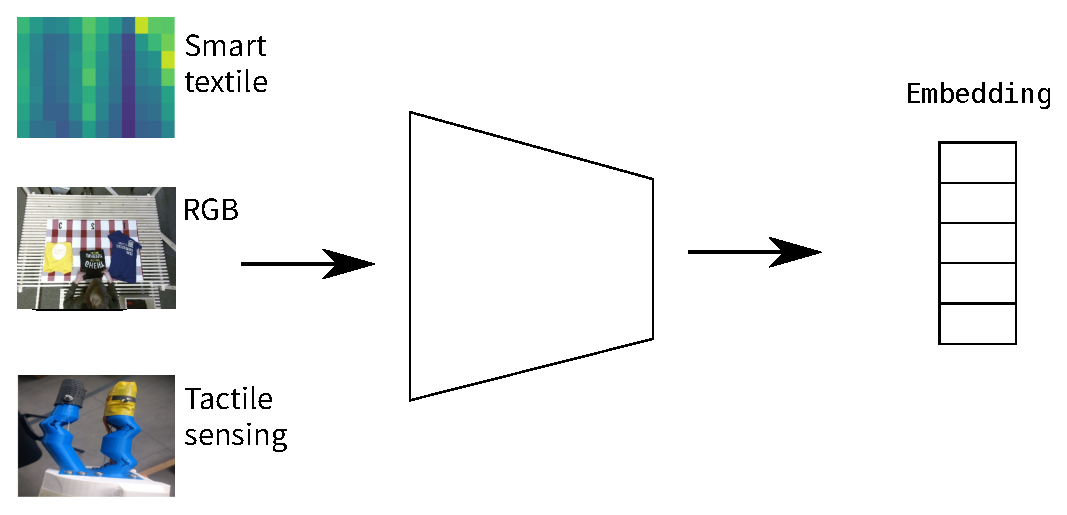
\includegraphics[width=\textwidth]{\home/chapters/08-conclusion/figures/ssr_nn_architecture_multimodal}
        \caption{Multiple modalities as input.}
        \label{fig:conc_tcn_multimodal}
    \end{subfigure}

    \caption[Multimodal contrastive embedding.]{Contrastive embedding trained with RGB images from different perspectives vs. trained with multiple modalities.}
    \label{fig:conc_multimodal_tcn}
\end{figure}

Generating meaningful representations when modalities can be dropped is an open research question. This question is of relevance for the smart textile we developed in \cref{ch:instrumentation}: it is impossible to instrument all clothing articles. We believe our multimodal contrastive learning approach proposed above holds merit in dealing with missing modalities on certain clothing items. Our idea is to train a multimodal embedding with instrumented clothing and tactile finger sensing in the way described above. At test time, non-instrumented cloth sensing can be swapped by images as we hypothesize that the embedding is trained to become invariant to the input modality to some extent. Although this does not eliminate the difficulty estimating the state caused by occlusions of the cloth self-collisions, we believe that this training procedure can enable the network to estimate to which sensor reading it should belong in embedding space.

We demonstrated our methodology in the context of task progression metrics for folding clothing. A next application is to use our work on learning progression metrics as reward functions for RL tasks. However, neural networks are easily fooled with adversarial examples \autocite{nguyen2015deep} and RL agents are known to exploit simulator and reward function dynamics. More generally, the problem of ensuring that a reinforcement learning agent's goal is aligned with our own goals is unsolved \autocite{Sutton2018}. However, we can aim to make our task progression metrics as robust as possible. One way to achieve more robustness is by adding a state machine to our framework, for example, by using \glspl{HMM}. An alternative can be found in the work of \textcite{borràs2020encoding} where a representation of the environment is embedded in a graph of manipulation primitives.

% Zie ook future outlook p23 van https://ieeexplore.ieee.org/abstract/document/922646
Loss functions are an important component for training neural networks as they determine the criteria for optimization. In this regard, future work can experiment and compare different existing loss functions like InfoNCE \autocite{oord2018representation} and cycle-consistency loss \autocite{Dwibedi2019cycle}.
Furthermore, new contrastive loss functions can be researched in order to learn a more fine-grained representation in the last stages of training. This is of relevance for cloth folding in order to distinguish between folding results with and without wrinkles.

Similar to research in the contrastive loss function, architectural design choices influence the performance of the embedding. This is due to borrowing a backbone neural network from supervised learning and appending transform heads on top of it. However, choosing the appropriate transform head is non-trivial. For example, we found that using a multi-layered transform head performed better than a single non-linear readout layer. This observation suggests that a potential area of research is the architectural design and tradeoffs associated with representation pretraining and how it compares to supervised learning.

A final, future avenue we propose comes in the form of the representation. Currently, our embedding is specified as a vector of scalar values. However, throughout this research we have stressed the difficulty of cloth state estimation due to self-occlusions. This uncertainty is something humans deal intuitively with. For example, we can implicitly construct a heatmap of the most likely places a folded corner of a cloth to be at. Similarly, a probabilistic embedding can denote a range of values and uncertainty about the encoding of the inputs to embedding space. This way, the inherent uncertainty of the state estimation can be taken into account in the reward function. This can be done by appending, Gaussian mixture layers on top of a base encoder network. The results discussed in \cref{ch:reward_functions}, then become to interpret the probability of being in a certain space in the embedding. \cref{fig:stoch_embd} demonstrates preliminary results when following a similar training approach with a probabilistic embedding. The benefit of this approach is that it naturally encodes uncertainty when not all information is available. This uncertainty is present in our folding dataset: when demonstrators fold, for example, a sleeve and return their hands, it is expected that they move their hands to the other side of the shirt to fold the other sleeve. However, sometimes the demonstrators return their hands to the same sleeve to further refine the fold. Such uncertainty can be modelled by, for example, a Gaussian mixture model containing multiple distributions in the mixture to express the input image is possibly at two places in embedding space. In addition to the benefit of modelling uncertainty in a domain where uncertainty is inherently present, a probabilistic approach integrates well within the paradigm of distributional RL where an agent receives a distribution of return rather than the expectation of this return \autocite{bellemare2017distributional}. It has been shown that learning a value distribution outperforms maximizing an expected return, especially in the presence of the instabilities caused by function approximators such as deep neural networks.

\begin{figure}[htpb]{}
    \centering
    \begin{subfigure}[b]{0.90\textwidth}
        \centering
        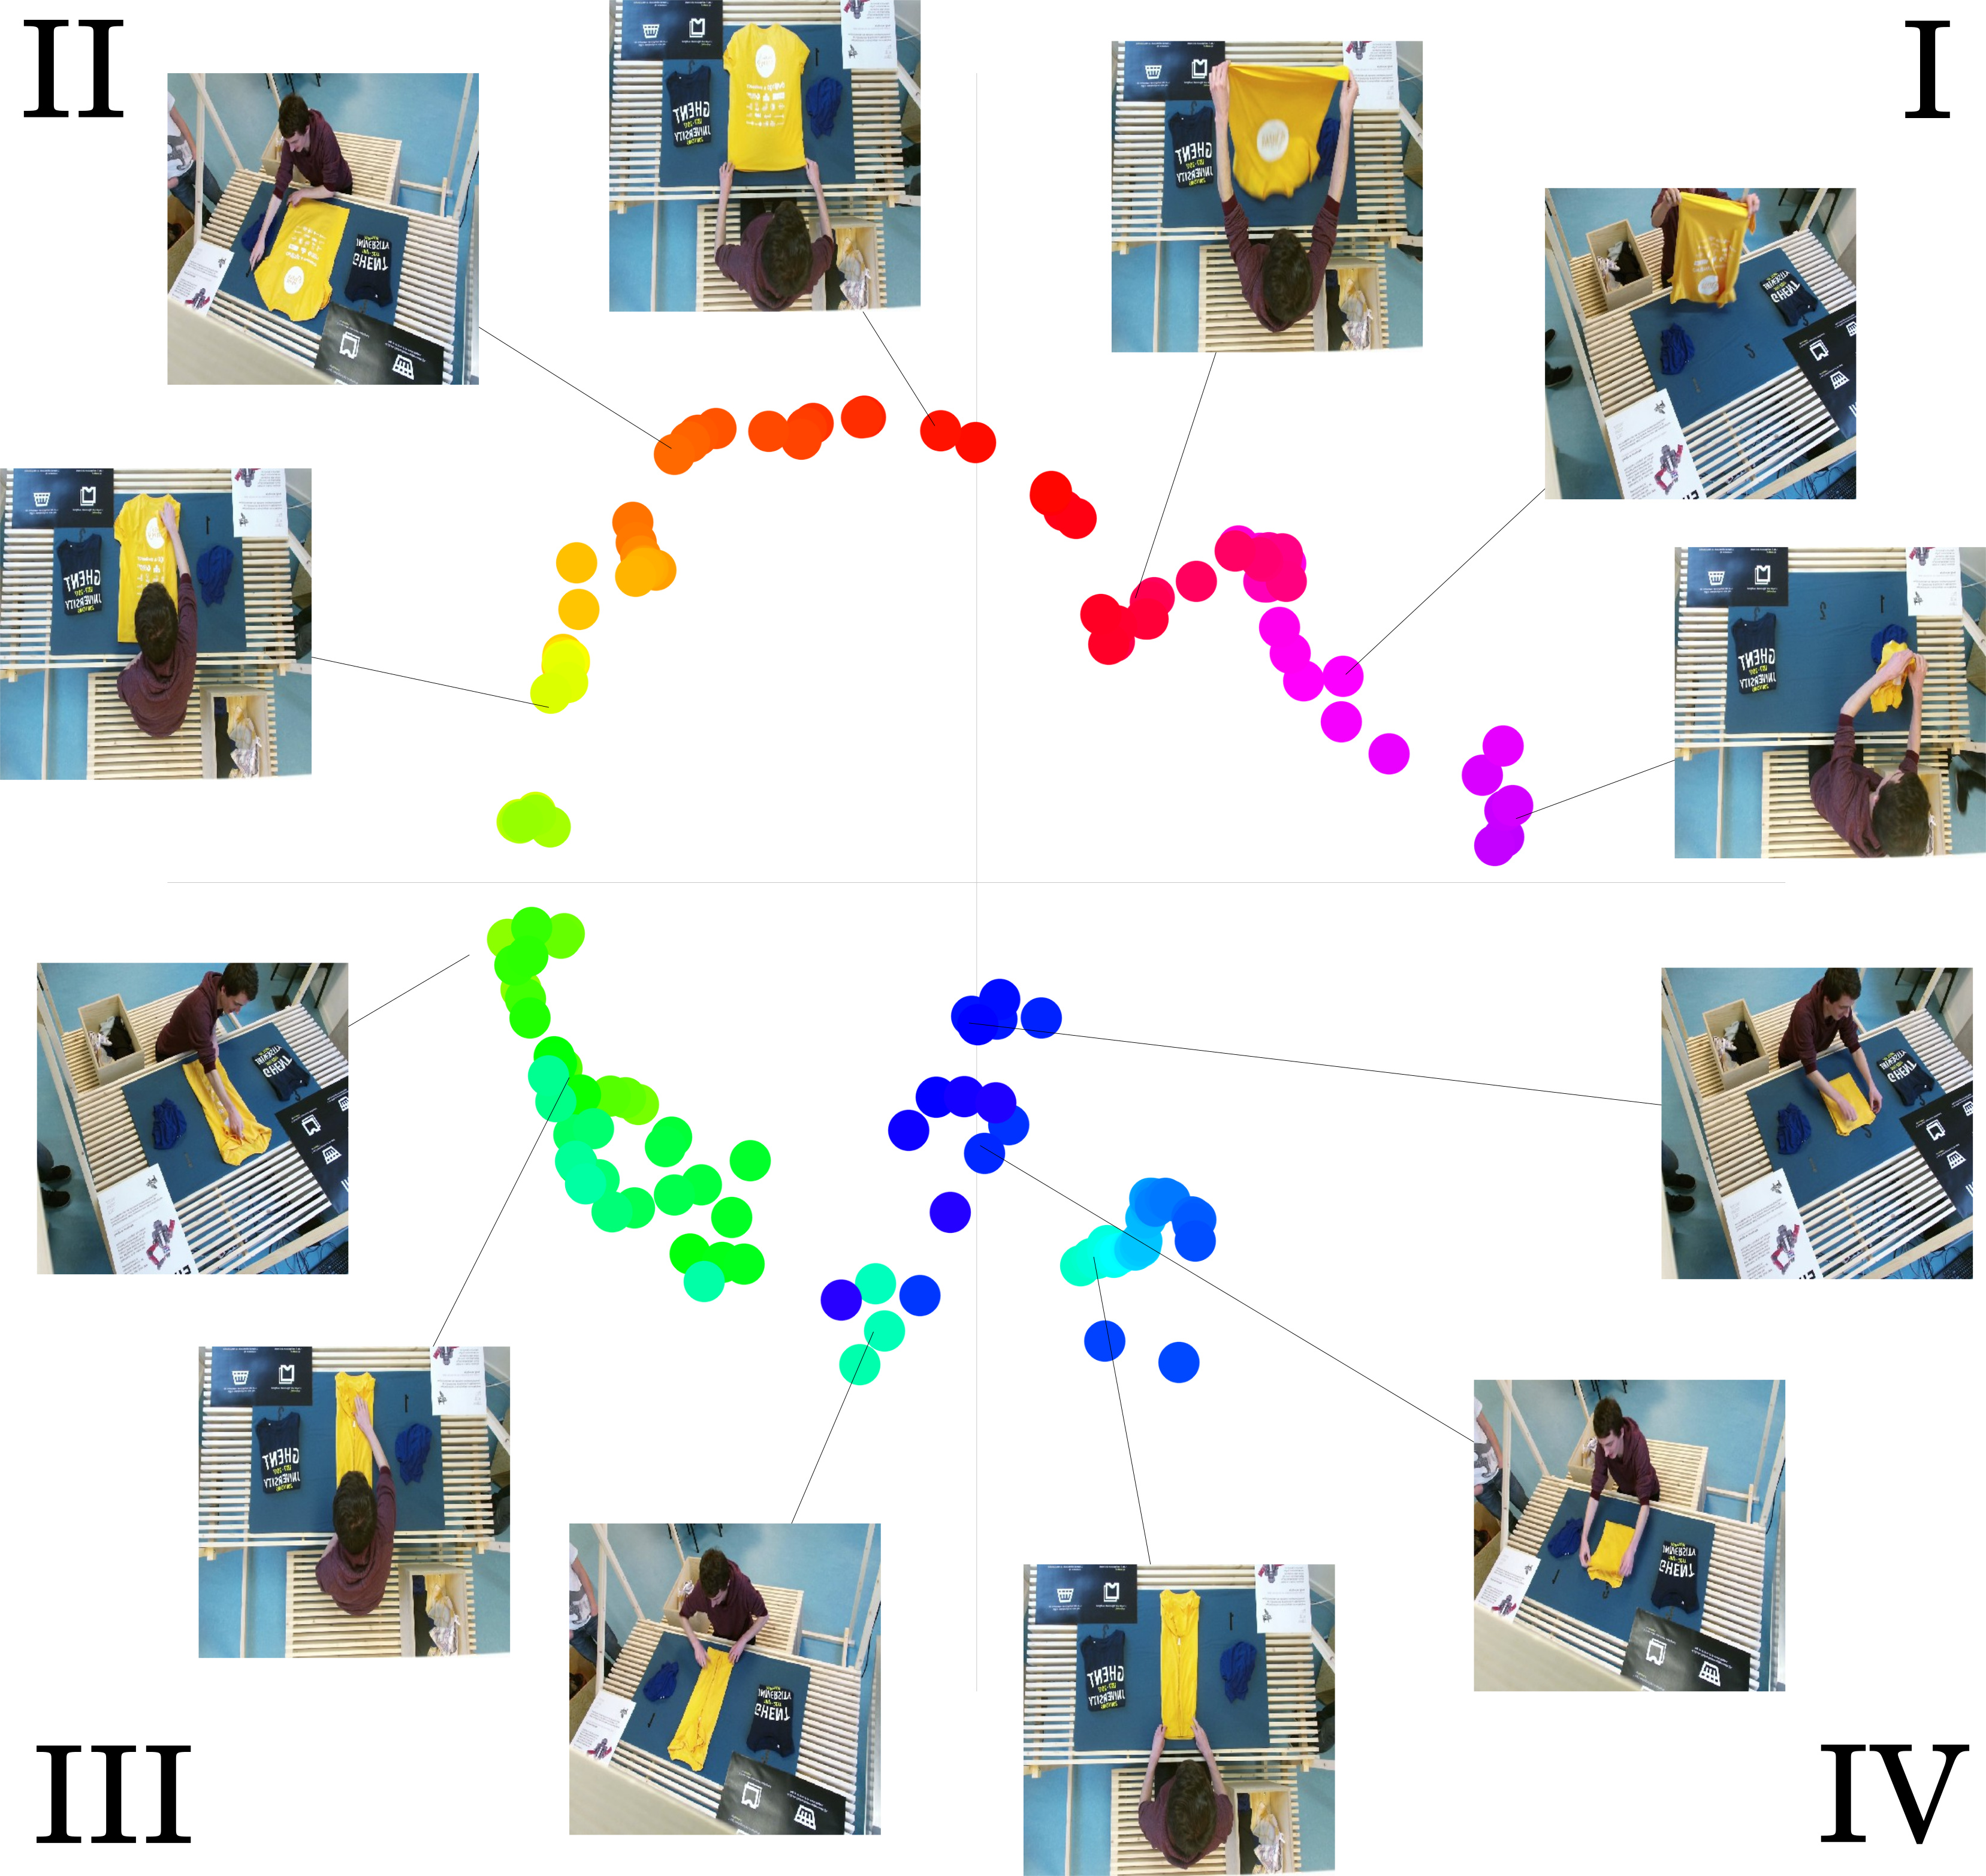
\includegraphics[width=\textwidth]{\home/chapters/08-conclusion/figures/umap.jpg}
        \caption{Deterministic embedding trained with the methodology of \cref{ch:reward_functions}. Note that this image contains a temporal dimension encoded in the color of the points.}
        \label{fig:determinstic_embd}
    \end{subfigure}
    \par\bigskip % force a bit of vertical whitespace
    \begin{subfigure}[b]{0.90\textwidth}
        \centering
        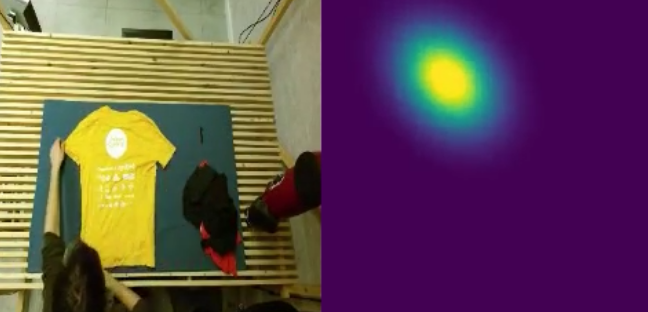
\includegraphics[width=\textwidth]{\home/chapters/08-conclusion/figures/prob_embd.png}
        \caption{Probablistic embedding trained with the methodology of \cref{ch:reward_functions}. The colors represent the probability of the image being in a certain part of the embedding space. Compared to the image above, this image shows the encoding of one image and does not encode a temporal dimension.}
        \label{fig:prob_embd}
    \end{subfigure}

    \caption[]{Deterministic vs. probabilistic embedding. A probabilistic embedding space allows expressing how certain the network is about the state of the environment.}
    \label{fig:stoch_embd}
\end{figure}

% SIMULATION:
%     Tuning physical parameters. Now wonky. Differentiable simulation for estimating physical parameters.
%     Massive in parallel with multiple robots. 

% TODO: epiloog? moet niet technisch zijn. Denk bv olivier: experimenten met planten is toch wel moeilijker dan ik dacht want planten sterven. 


% Epiloog brainstorm
%  start end2end with many failed experiments 
% When I started, many articles about self-driving cars, robots taking over our jobs. I found this to be in stark contrast with how i experienced my research. How will this clumsy Baxter cook my dinner? Will Tesla really deploy this neural network that believes the picture of this dog is a cat by changing a single pixel? 
% I believe the field is gradually passing the top of the Gartner Hype cycle. 
% It was very hard to not jump at the latest, craziest deep RL method. 


\end{document}
